%   Filename    : chapter_3.tex 
\chapter{Research Methodology}
\label{sec:methodology}

This chapter discussed the materials and methods employed in the study, focusing on the development requirements, as well as the software and programming languages utilized. It also detailed the overall workflow in conducting the study, Morphometric-Based Non-Invasive Sex Identification of Blood Cockles \textit{Tegillarca granosa} (Linnaeus), 1758) using machine learning and deep learning technologies.

Dr. Victor Emmanuel Ferriols, the director of the Institute of Aquaculture, oversaw the overall workflow and conduct of the experiment. The researchers were also guided by research associates LC Mae Gasit and Allena Esther Artera. Consequently, the entire dataset collection process was conducted at the University of the Philippines Visayas hatchery facility.

The methodology consisted of nine parts: (1) Sample Collection, (2) Ethical Considerations, (3) Creating \textit{T.granosa} Dataset, (4) Morphological Characteristics Collection (5) Image Acquisition and Pre-processing, (6) Hardware and Software Configuration,(7) Morphometric Characteristics Evaluation Using Machine Learning, (8) Morphological Characteristics Evaluation Using Deep Learning, and (9) Evaluation Metrics

\section{Sample Collection}
\label{sec:samplecollect} 

The collection of \Tgranosa samples used in this study was part of an ongoing research project by UPV DOST-PCAARRD titled "Establishment of the Center for Mollusc Research and Development: Development of Spawning and Hatchery Techniques for the Blood Cockle (\textit{Anadara granosa}) for Sustainable Aquaculture." A total of 271 samples were provided for this study to classify the sex of \textit{T. granosa}. The samples, ranging in size from 34 to 61 mm, were sourced from the coastal area of Zaraga, Iloilo, and fish markets in Ivisan, Capiz, Philippines (\textit{see Figure~\ref{fig:granosa_shells}}).

The research and experimentation were conducted at the University of the Philippines Visayas hatchery facility in Miagao, Iloilo, where the samples were maintained in 200 L fiberglass-reinforced plastic (FRP) tanks containing filtered seawater with 35 ppt salinity \cite{miranda2023}.

As part of the data collection process, the researchers utilized induced spawning and dissection to classify the sex of the samples. Induced spawning through temperature fluctuations was the most natural and least invasive method for bivalves compared to other approaches \cite{aji}. However, since not all samples exhibited gamete release, the researchers also performed dissections, assisted by hatchery staff, to expedite data collection. The sex of the dissected samples was identified based on the coloration of gonad tissue, which varies according to sex and maturity stage. Females exhibited orange-red to pale orange gonads, while males displayed white to grayish-white gonads \cite{may2021}.

The methods used for data collection were considered noninvasive, particularly given that \Tgranosa are oxygen regulators well adapted to tidal exposure and hypoxia \cite{davenport1986}.

\begin{figure}[!htbp]
	\centering
	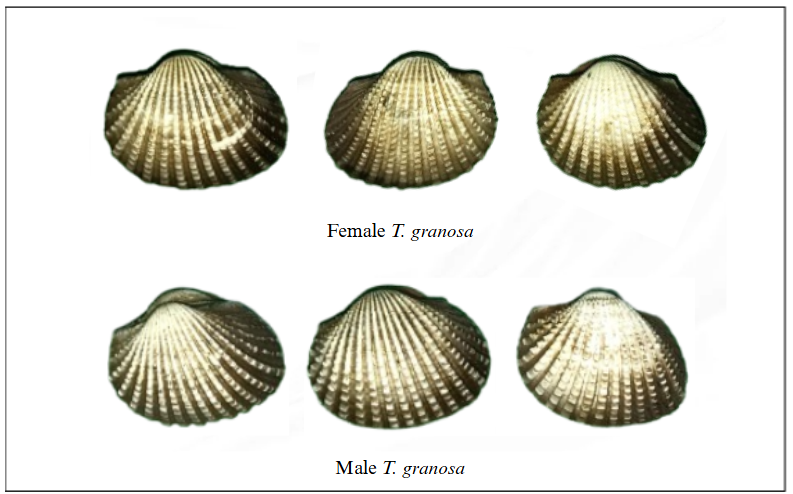
\includegraphics[width=0.9\textwidth]{figures/male-female T.granosa.png}
	\caption{Male and Female \Tegillarcagranosa shells}
	\label{fig:granosa_shells}
\end{figure}

\section{Ethical Considerations}
\label{sec:ethical}

The ongoing research project titled "Establishment of the Center for Mollusc Research and Development: Development of Spawning and Hatchery Techniques for the Blood Cockle (\textit{Anadara granosa}) for Sustainable Aquaculture"—from which the samples used in this study were obtained—was reviewed and approved by the Institutional Animal Care and Use Committee (IACUC) of the University of the Philippines Visayas. 

\section{Creating \textit{T. granosa} Dataset}
\label{sec:dataset}

The experiment began with the collection of preliminary observations from 100 \Tgranosa samples. For the actual experimentation, the researchers collected the full dataset in batches until a total sample size of 271 \Tgranosa was reached. Linear measurements—including width, height, length, rib count, hinge line length, and the distance between the umbos—were recorded and organized into a CSV file. This dataset served as the foundation for training and testing machine learning models, as well as for establishing a baseline for the Convolutional Neural Networks.

Images of each sample were captured and saved in JPG format using a standardized file naming convention that included the sample's sex, the shell's orientation or view, and its corresponding number out of the 271 total samples. File names for female \Tgranosa samples began with “0”, while those for male samples began with “1”. Each file name also included one of the six captured views: (1) dorsal, (2) ventral, (3) anterior, (4) posterior, (5) left lateral, and (6) right lateral (refer to Figure~\ref{fig:granosa_views}), followed by a unique sample number. For example, “010001” denoted the first female sample taken from the dorsal view, while “110001” represented the first male sample from the same view. This naming convention was implemented to prevent data leakage and ensure accurate labeling of images according to their respective samples.

\begin{figure}[!htbp]
	\centering
	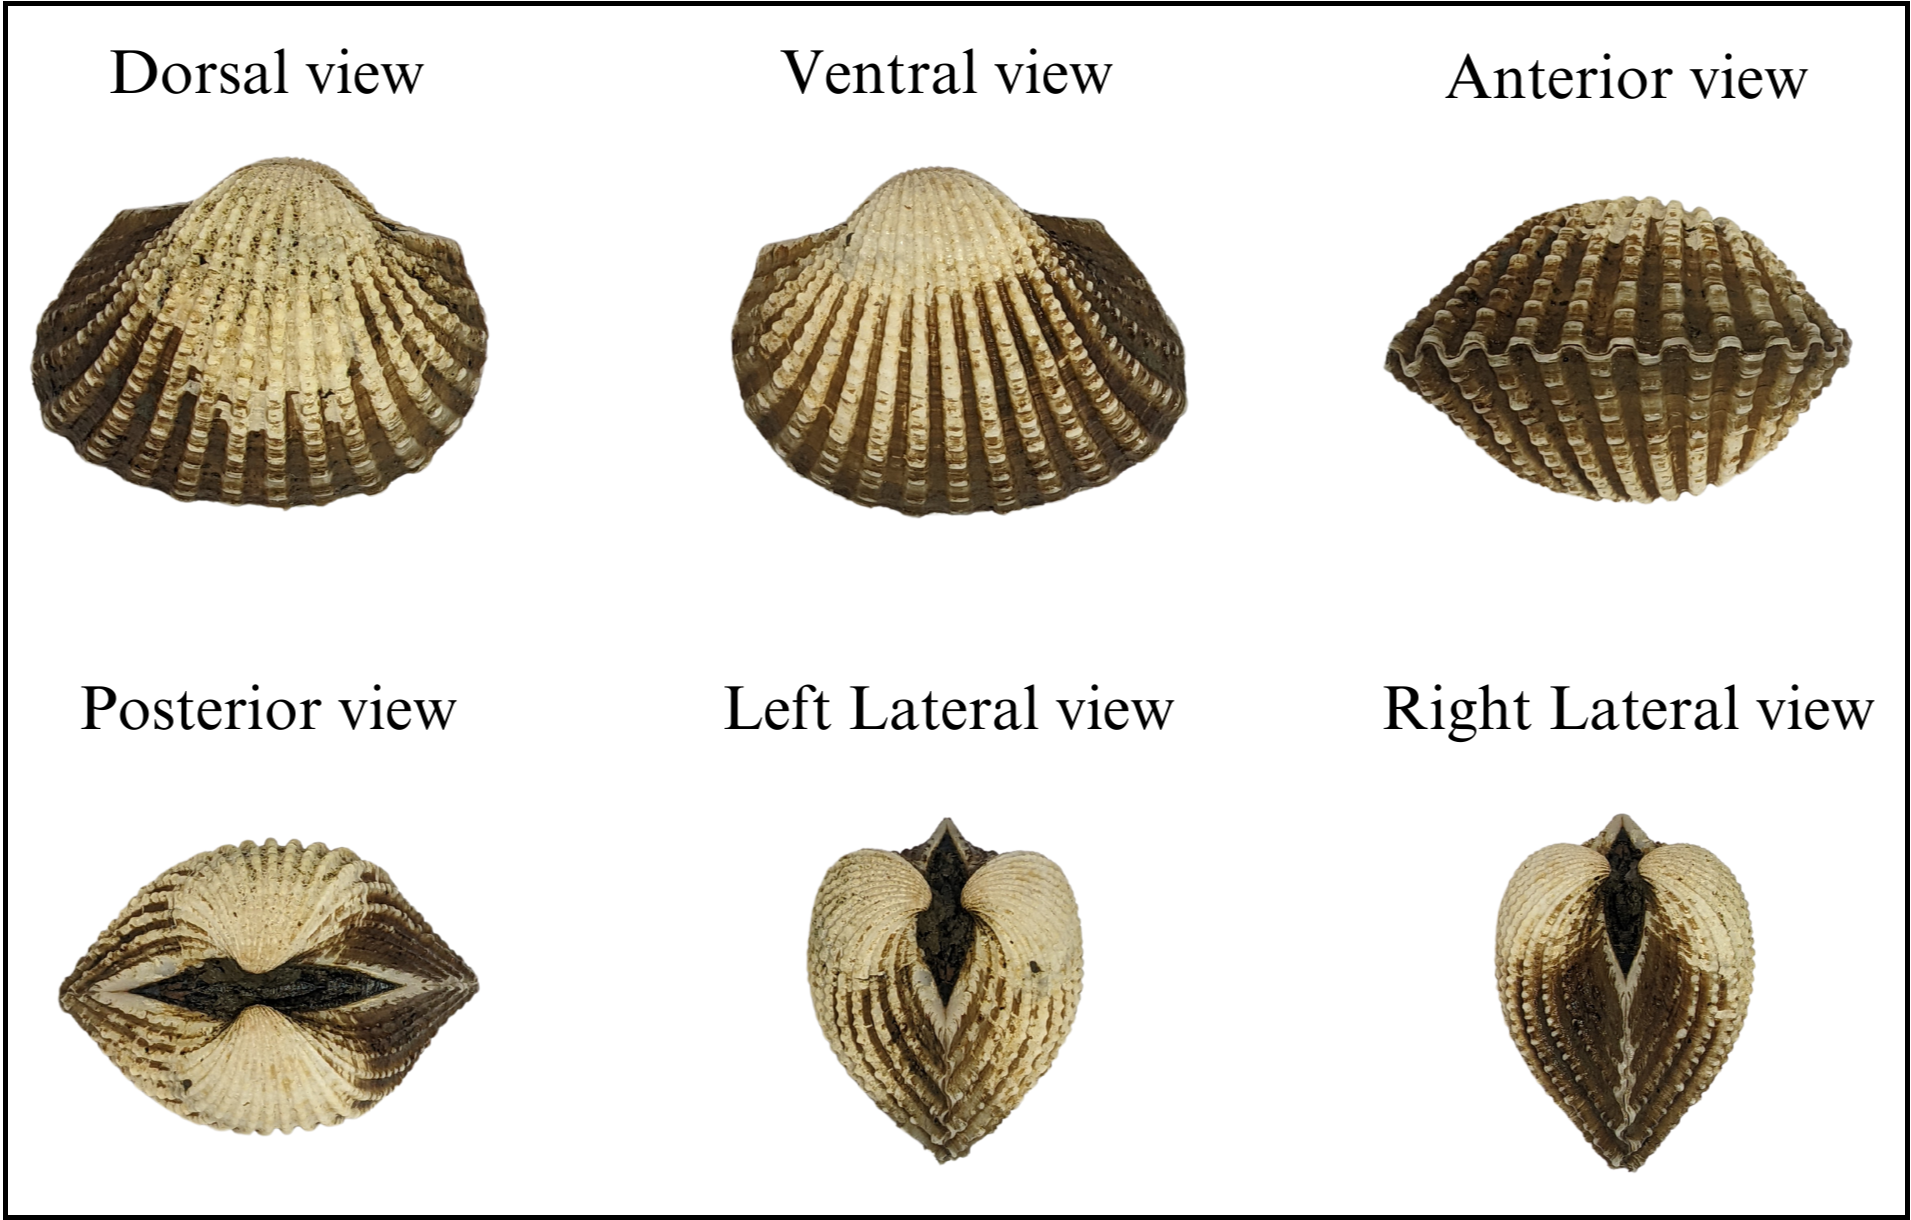
\includegraphics[width=0.9\textwidth]{figures/view.png}
	\caption{Different Views of the \textit{T. granosa} Shell Captured}
	\label{fig:granosa_views}
\end{figure}

\newpage
\section{Morphological and Morphometric Characteristics Collection}
\label{sec:morphochar}

Morphology refers to biological form and is one of the most visually recognizable phenotypes across all organisms \cite{tsutsumi2023}. In this study, morphological characteristics describe the structural features of \textit{T. granosa}, focusing on measurable attributes such as shape, size, and color. Morphometric characteristics, on the other hand, refer to specific quantifiable features of T. granosa, including length, width, height, hinge line length, distance between the umbos, and rib count. As stated by the researchers, quantifying and characterizing these traits is essential for understanding and visualizing variations in \Tgranosa morphology.

The researchers measured the height, width, and length of \Tgranosa using a Vernier caliper with a precision of up to 0.01 mm. Refer to Figure~\ref{fig:linear_measurements} for the corresponding measurement diagram. Length (A) refers to the distance from the anterior to the posterior of the shell. Width (B) is defined as the widest span across the shell from the left to the right valve. Height (C) measures the distance from the base to the apex of the shell. In addition, the hinge line length (D) near the hinge and the distance between the umbos (E) were recorded.

Reyment and Kennedy (1998) emphasized that including rib count as supplementary information can enhance identification accuracy. Following this insight, the researchers also recorded the rib count for both male and female \textit{T. granosa}, adjusting the values by calculating ratios to account for natural size variation among specimens.

\begin{figure}[!htbp]
	\centering
	\includegraphics[width=0.95\textwidth]{figures/Tegillarca_granosa_linear_measurements.png}
	\caption{Linear Measurements of  \Tegillarcagranosa shell.}
	\label{fig:linear_measurements}
\end{figure}

\section{Image Acquisition and Data Gathering}
\label{sec:imageprocess}

This study comprised 144 male and 127 female \Tgranosa samples, resulting in a total of 1,626 images captured from various angles. To ensure consistency during image acquisition, the researchers constructed a box-like structure with a white background to control the imaging environment. This setup allowed for uniform image captures by fixing the camera at a consistent angle directly above the \textit{T. granosa}. A ring light was positioned in front of the box to enhance image quality, eliminate shadows, and ensure clarity of the samples throughout the image acquisition process.

The images were captured using a Google Pixel 3 XL smartphone, which features a resolution of 2960 × 1440 pixels and a 12.2 MP camera (4032 × 3024 pixels). Additional camera specifications include an f/1.8 aperture, 28mm wide lens, ½.55” sensor size, 1.4µm pixel size, dual-pixel phase detection autofocus (PDAF), and optical image stabilization (OIS) \cite{concepcion2023}.

\begin{figure}[!htbp]
	\centering
	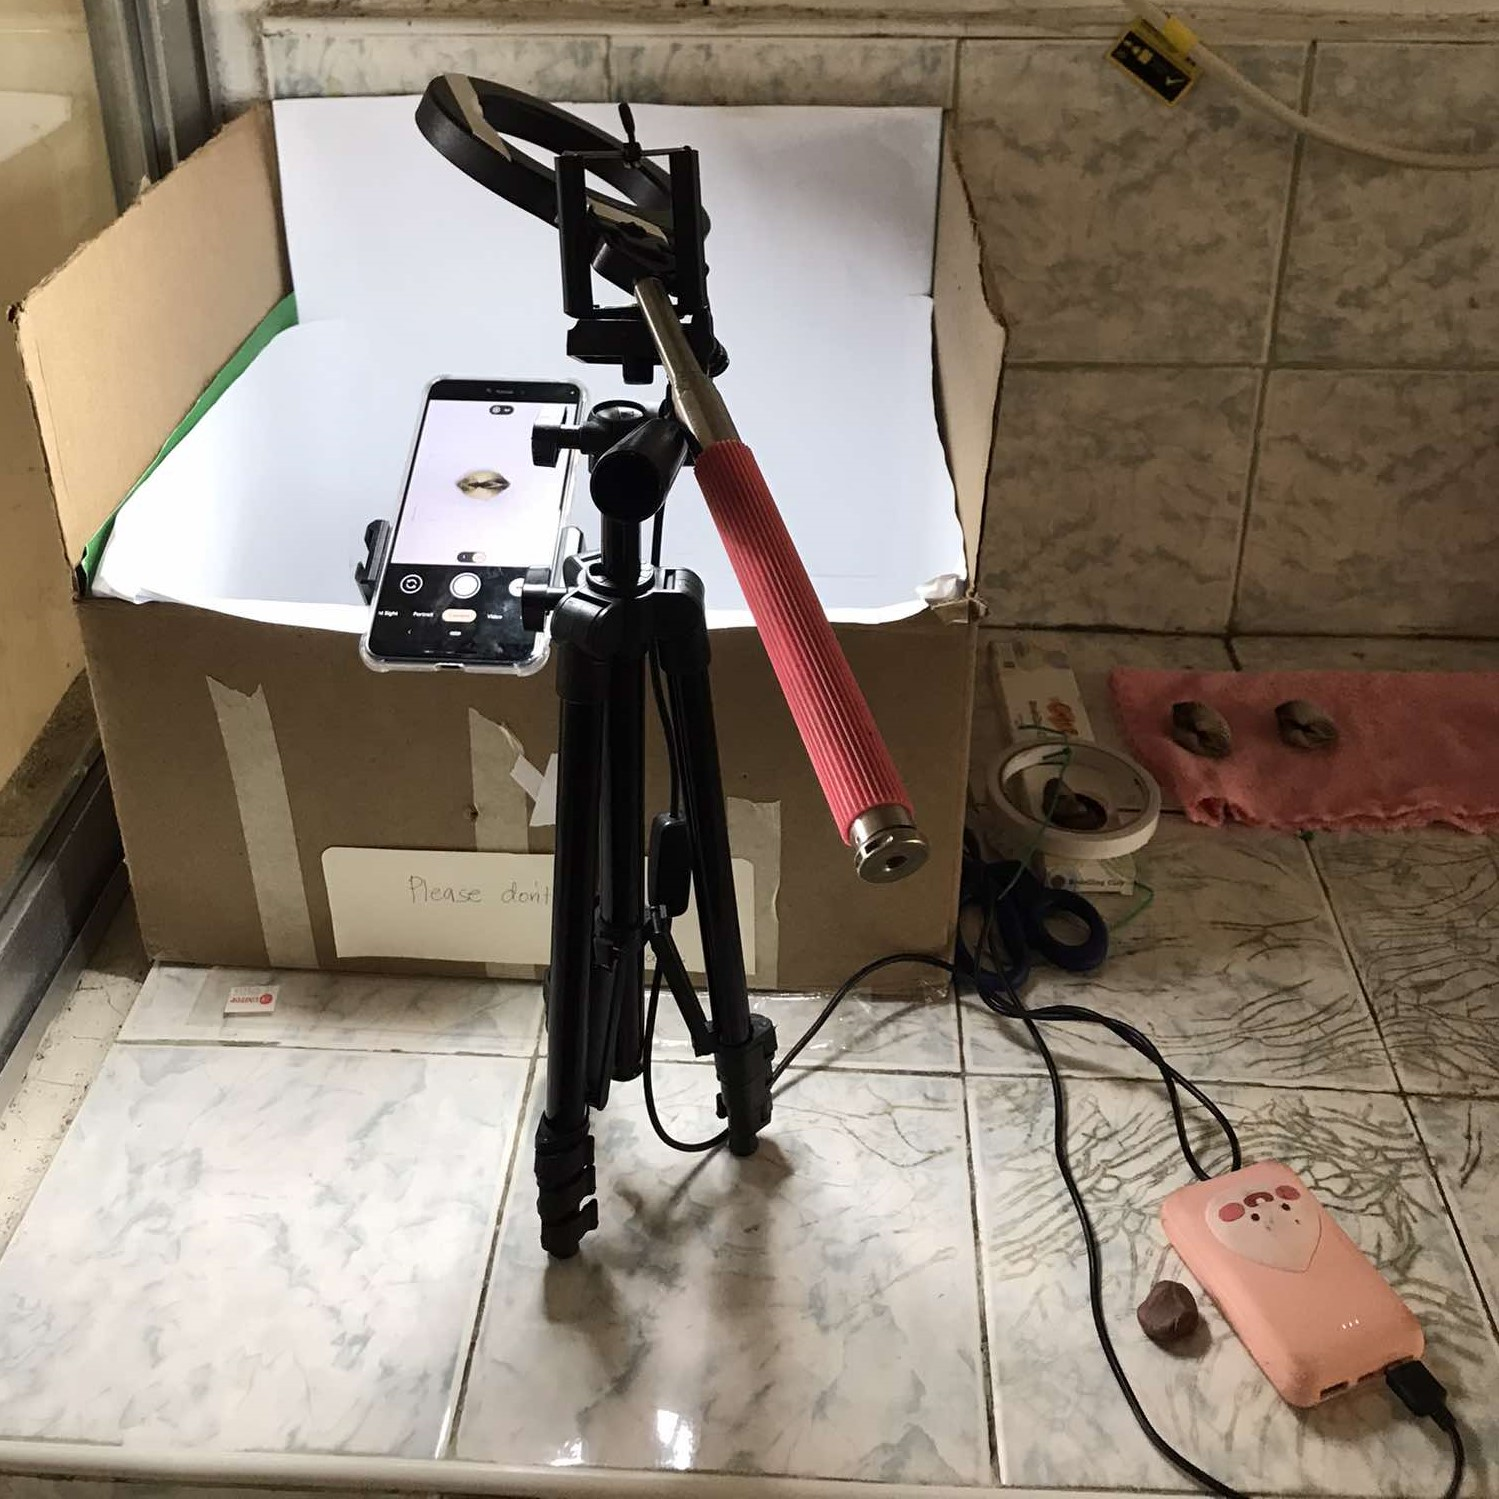
\includegraphics[width=0.4\textwidth]{figures/setup.jpg}
	\caption{Image Acquisition Setup for \textit{T. granosa} Samples}
	\label{fig: setup}
\end{figure}

\newpage
\section{Hardware and Software Configuration}

This section of the paper discusses the software, programming languages, and tools used for sex identification. Data collection, preprocessing, and model training were conducted on a Windows 11 operating system using an ACER Aspire 3 general-purpose unit (GPU) equipped with an AMD Ryzen 3 7320U CPU with Radeon Graphics (8 cores) @ 2.395 GHz and 8 GB of RAM. Google Colaboratory was utilized for collaborative preprocessing, computer vision tasks, and model training. Image preprocessing was performed using computer vision techniques in Python, while machine learning and deep learning models were developed using Python libraries, including Keras. The results of the gathered measurements were stored and managed using spreadsheet software. GitHub was employed for version control, documentation, and activity tracking throughout the study.

\section{Morphometric Characteristics Evaluation Using Machine Learning }
\label{sec:ml models}

This section of the paper discusses the machine learning operations that served as a baseline prior to implementing more complex deep learning methods for image classification. The study utilized collected variables including linear measurements—length, width, height, hinge line length, distance between the umbos, and rib count—along with derived features used as predictors. These included the length-to-width ratio, length-to-height ratio, width-to-height ratio, umbo distance-to-length ratio, hinge line length-to-length ratio, umbo distance-to-height ratio, and rib density. The samples were classified by sex, with females labeled as 0 and males as 1, which served as the response variable.

\subsection{Data Preprocessing}
\label{sec:pre-processing}

\begin{figure}[!htbp]
	\centering
	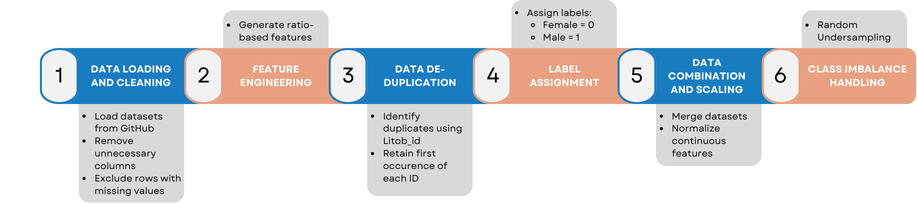
\includegraphics[width=1\textwidth]{figures/pipeline.png}
	\caption{Data Preprocessing Pipeline}
	\label{fig:pipeline}
\end{figure}

The preprocessing of the dataset involved several essential steps, carried out using Python in Google Colaboratory, in preparation for machine learning analysis (see Figure~\ref{fig:pipeline}).

\textbf{\textit{Data Loading and Cleaning}}

The process began by loading two separate datasets for male and female \textit{T. granosa} directly from GitHub using \texttt{pd.read\_csv()}. Unnecessary columns were removed, and rows containing missing values were excluded using the \texttt{dropna()} function to ensure data completeness and reliability.

\textbf{\textit{Feature Engineering}}

Additional ratio-based features were generated to augment the existing measurements. These included the length-to-width ratio, length-to-height ratio, width-to-height ratio, hinge line length-to-length ratio, umbos distance-to-length ratio, umbos distance-to-height ratio, and rib density. These derived features aimed to emphasize shape characteristics independent of size, improving the models' ability to distinguish morphological differences between sexes.

\textbf{\textit{Data De-duplication}}

To avoid redundancy and ensure each specimen was uniquely represented, the last three digits of each \texttt{Litob\_id} were used to identify duplicates. Only the first occurrence of each unique ID was retained, reducing potential bias caused by repeated entries.

\newpage
\textbf{\textit{Label Assignment}}

A new column labeled \texttt{Label} was added to both datasets. Female specimens were assigned a label of 0, and male specimens a label of 1. This column served as the target variable for classification.

\textbf{\textit{Data Combination and Scaling}}

After cleaning and feature engineering, the male and female datasets were merged into a single DataFrame. The \texttt{Litob\_id} column was removed post de-duplication. All continuous numeric features were normalized using \texttt{MinMaxScaler} to scale values to the range [0, 1].

Rib count was excluded from normalization because it is a discrete feature with biologically meaningful bounds. According to best practices in machine learning, normalizing discrete or categorical features can distort their meaning and is often unnecessary \cite{jaiswal2024}. In this study, rib count was treated as a categorical attribute due to its biological significance and finite, non-continuous nature.

\textbf{\textit{Class Imbalance Handling}}

After normalization, class imbalance was addressed by applying Random Under-sampling to the male dataset. This technique randomly reduced the number of male samples to match the number of female samples (127 each), ensuring equal class representation. By using this approach, model bias was minimized, and the classification performance became more reliable across both classes.

\subsection{Machine Learning Models Training}

\textbf{\textit{Model Selection and Hyperparameter Tuning}}

To establish a baseline for classification, various models were evaluated: Logistic Regression, K-Nearest Neighbors, Support Vector Machine, Random Forest, AdaBoost, Extra Trees, and Gradient Boosting. Hyperparameter tuning was conducted using \texttt{GridSearchCV}, which systematically identified the optimal settings for each model to enhance accuracy and performance.

\textbf{\textit{Cross-Validation}}

A five-fold cross-validation approach was implemented. The dataset was divided into five subsets, with four used for training and one for testing. This process was repeated five times, with each fold serving as the test set once. This method ensured that model evaluation was robust and generalizable, minimizing the bias that may result from a single train-test split. \cite{geeksforgeeks2024}

\begin{figure}[!htbp]
	\centering
	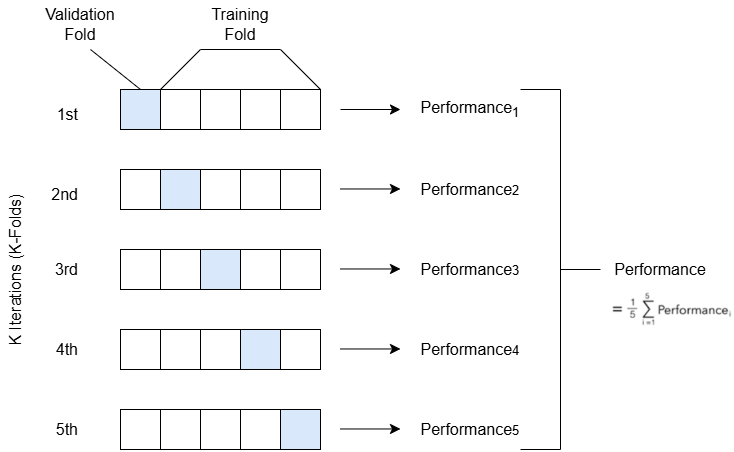
\includegraphics[width=0.8\textwidth]{figures/cv.png}
	\caption{Diagram of k-fold cross-validation with k = 5}
	\label{fig: cv}
\end{figure}

\section{Morphological Characteristics Evaluation Using Deep Learning}
This section outlines the application of deep learning techniques in analyzing the morphological characteristics of \textit{Tegillarca granosa} to identify their sex based on shell images. A Convolutional Neural Network (CNN) architecture was implemented and trained on preprocessed images using cross-validation.

\textbf{\textit{Image Preprocessing}}

This subsection details the image processing techniques applied to raw shell images of \Tgranosa using computer vision methods before training the deep learning model. The image preprocessing techniques include standardizing input dimensions and removing shadows, background, and noise. Each image underwent data augmentation to enhance feature visibility for effective learning. Image preprocessing ensures consistent and high-quality input data for model training.

\textbf{\textit{Adjusting Dimensions}}

All images were resized to a consistent dimension of 256x256 pixels to ensure uniformity throughout the dataset. This standardization is essential for Convolutional Neural Networks (CNNs), as a consistent input dimension is required. While resizing, the aspect ratio was maintained to prevent distortion of the morphological features, and padding was added to retain the original format.

\textbf{\textit{Background Removal}}

Background removal was performed to maintain a consistent white background throughout the dataset. The tool \texttt{rembg} was used to efficiently remove the original background, retaining the foreground from the raw images. This method resulted in clear images with a white background, enhancing focus on the morphological features and defining the shell boundaries.

\textbf{\textit{Shadow Removal}}

To minimize noise caused by shadows around the shell, HSV thresholding, contours, and morphological thresholds were applied to isolate and remove shadowed regions. This approach preserved the natural color of the blood cockles and eliminated shadows and noise from the surrounding area.

\begin{figure}[h]
	\centering
	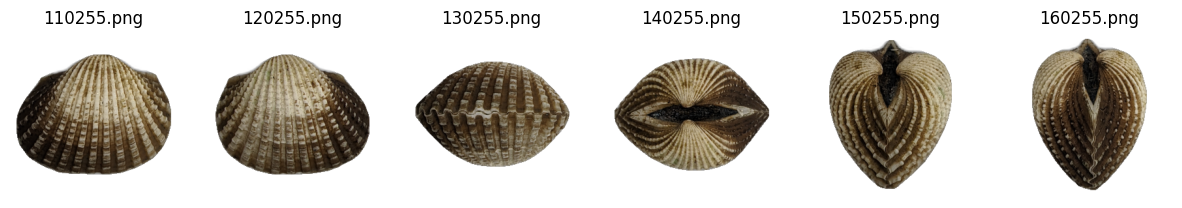
\includegraphics[width=\textwidth]{figures/male_shadows_removed.png}
	\caption{Shadows removed from male samples at different angles}
\end{figure}

\begin{figure}[h]
	\centering
	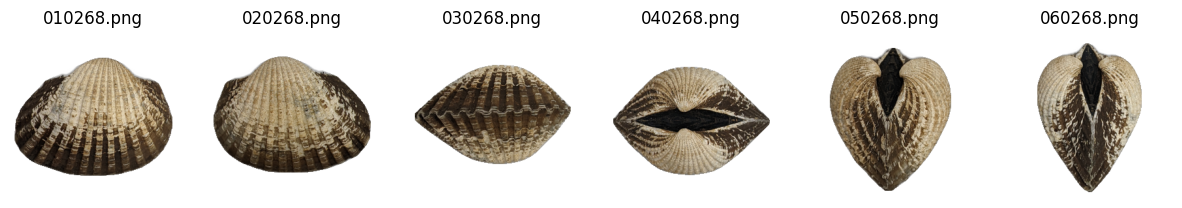
\includegraphics[width=\textwidth]{figures/female_shadows_removed.png}
	\caption{Shadows removed from female samples at different angles}
\end{figure}

\subsection{Convolutional Neural Network}

Convolutional Neural Networks are the main deep learning tool used in image classification, specifically binary classification. CNNs leverage their ability to share weights and use pooling techniques, reducing the number of parameters \cite{cui2020}. The proposed CNN architecture for sex identification of blood cockles employs 12 layers designed to extract features from the input image with dimensions of (256, 256, 3). The layers consist of four convolution layers, a flatten layer, and two dense layers. The CNN framework used in this study is shown in Figure~\ref{fig:cnn_architecture}.

\begin{figure}[h]
	\centering
	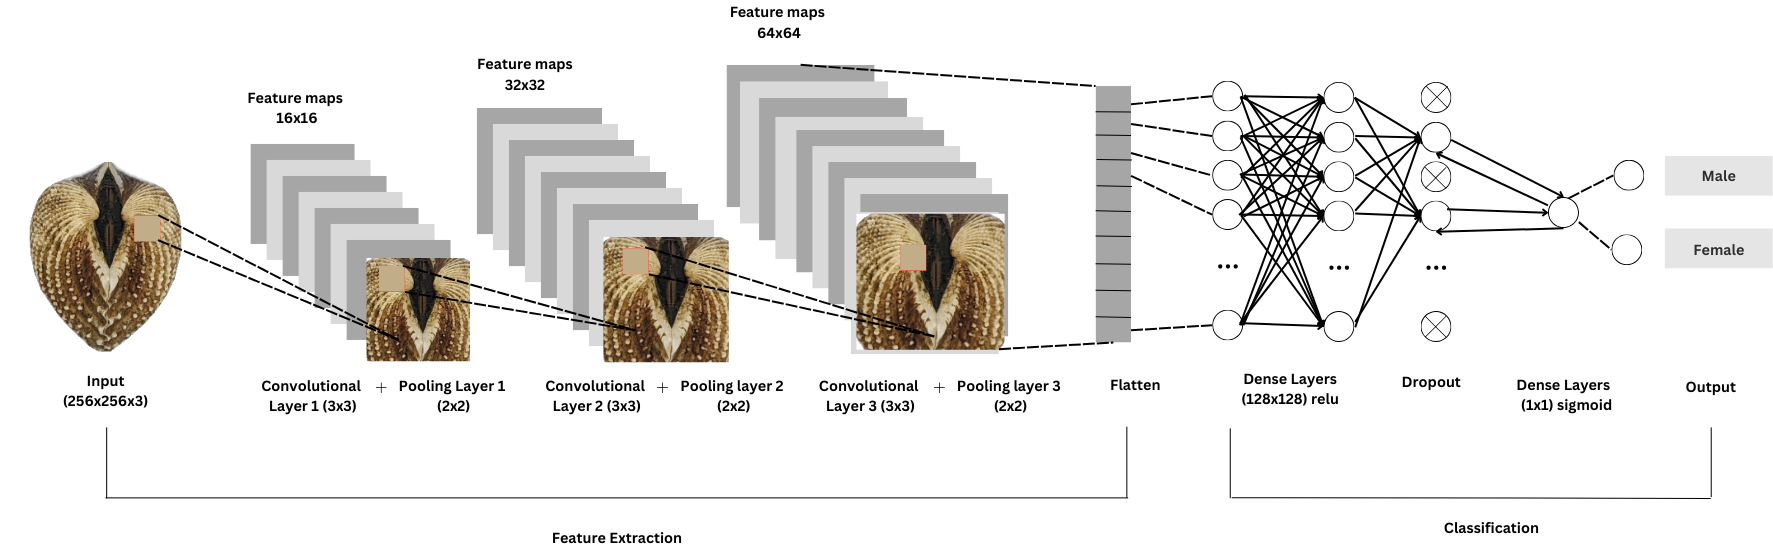
\includegraphics[width=\textwidth]{figures/cnn_architecture.png}
	\caption{Architecture of Convolutional Neural Network (CNN)}
	\label{fig:cnn_architecture}
\end{figure}

\textbf{\textit{Convolution Layer}}

The convolution layers of CNN extract the features from the input image through the convolution operation. This study uses four convolution layers with a 3x3 kernel size and filter sizes of 16, 32, 64, and 128. The first layer extracts the low-level features, such as edges, lines, and corners, while the deeper layers iteratively extract more complex information from these low-level features. The ReLU activation function was used, allowing the model to learn the complex patterns within the data.

\textbf{\textit{Pooling Layer}}

A pooling layer was added after the convolution layer to enhance calculation speed and prevent overfitting \cite{cui2020}. In this study, max pooling was applied with a (3,3) kernel size.

\textbf{\textit{Fully Connected and Dropout}}

Fully connected layers follow after the convolution and pooling layers. Each neuron connects to all neurons of the previous layer. The output values from the fully connected layers are sent to an output layer. It was classified using different sigmoid functions appropriate for binary classification.

A large number of parameters in the training process can lead to overfitting. It occurs when the model learns the training data too well, including its noise and irrelevant details. This results in poor performance on unseen data. To mitigate the overfitting, the dropout layer was employed. Dropout works by temporarily discarding a portion of the neurons in the network with probability \( p \) (\( 0 < p < 1 \)). During this process, these neurons do not participate in the forward propagation process of CNN and the backward propagation process \cite{cui2020}.

\subsection{CNN Training}
The dataset consists of 1626 samples, with 127 samples from females and 144 samples from males, individually for each angle. Given the minimal class imbalance, random undersampling was carried out to create a balanced dataset. All images were resized to 256x256 pixels and normalized using a Rescaling layer, ensuring pixel values were within the range [0, 1].

\textbf{\textit{Data Splitting}}

Due to the limited dataset size, a traditional train-test split was not adopted. Instead, a 5-fold stratified cross-validation approach was used to maximize the use of available data while preserving the class distribution within each fold. \texttt{StratifiedKFold} was applied to ensure that the distribution of male and female samples remained consistent across all folds, thereby enabling fair and robust model evaluation \cite{stratifiedKFold2020}.

\begin{figure}[h]
	\centering
	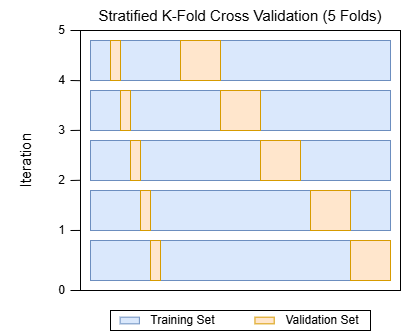
\includegraphics[width=0.8\textwidth]{figures/skf.png}
	\caption{Diagram of stratified k-fold cross-validation with k=5}
\end{figure}

\textbf{\textit{Data Augmentation}}

Before model training, online data augmentation was applied exclusively to the training data within each fold, creating new data variations on the fly. The augmentations included random horizontal flips, slight rotations, and zoom transformations to enhance data diversity and improve model generalization \cite{awan2022}. All augmentation was strictly applied only to the training subset of each fold to prevent data leakage and maintain the validity of the results. On-the-fly data augmentation (OnDAT) generates augmented data during each iteration, exposing the model to constantly changing data variations. Augmenting the original data allows better exploration of the underlying data generation process and has the potential to prevent the model from overfitting spurious patterns, thereby improving performance \cite{cerqueira2024}.

\begin{figure}[h]
	\centering
	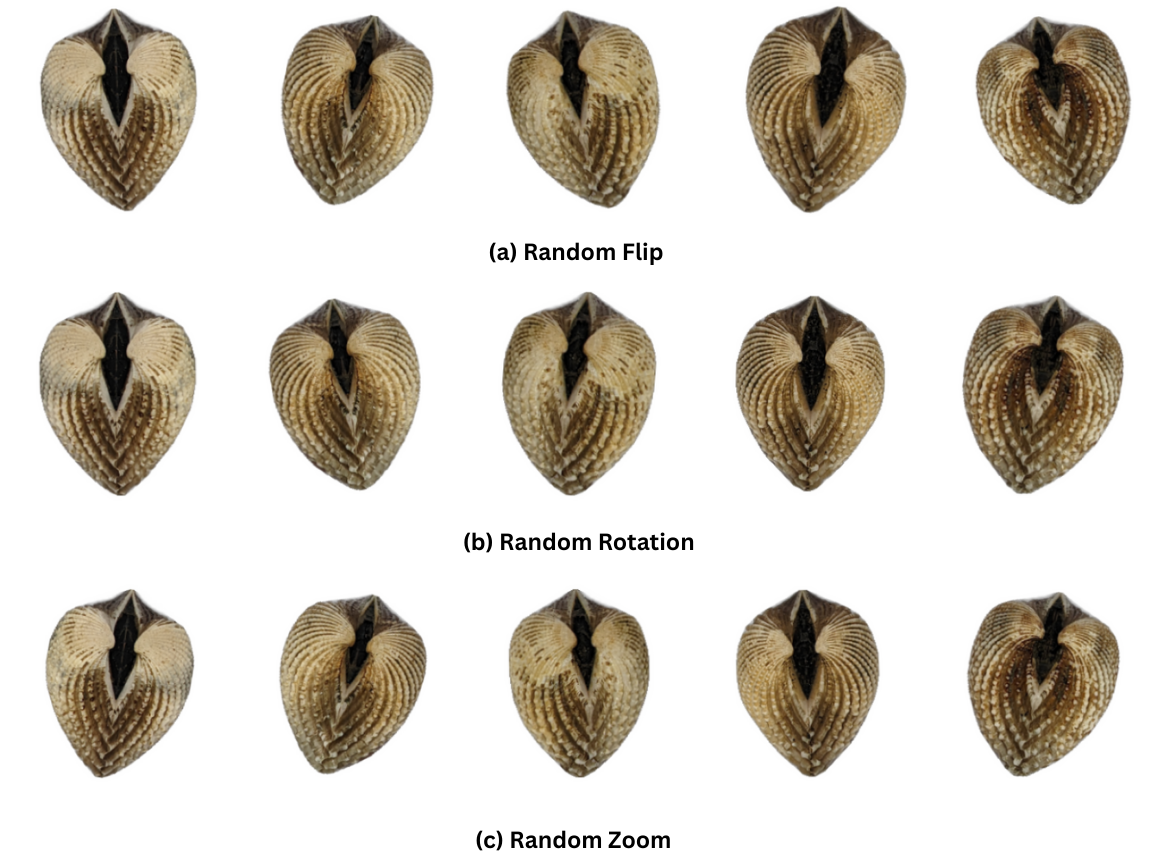
\includegraphics[width=\textwidth]{figures/data_augmentation.png}
	\caption{Data Augmentation Techniques}
\end{figure}

\textbf{\textit{Training Procedure}}

During the training process, model performance per fold was carefully monitored. One important thing to observe is the consistency in the performance, whether the model is still learning or is at high risk of overfitting. Early stopping was applied to ensure the stable performance of the model across folds. This technique allows for monitoring the training of the neural network, stopping when the performance metrics, in this case, validation loss, cease to improve. Furthermore, to enhance the learning process, \texttt{ReduceLROnPlateau} was applied, which decreased the learning rate if there was no improvement in the model for a specified number of epochs \cite{kerasTeam}.

The model was trained using the Adam optimization algorithm, with an initial learning rate of 0.001. Binary cross-entropy, commonly known as the log loss, was employed as the loss function due to its effectiveness in binary classification tasks. To reduce the risk of overfitting, a dropout rate of 0.5 was applied, randomly deactivating half of the neurons during the training process to improve generalization.

\section{Evaluation Metrics}
Evaluating the performance of a binary classification model is essential, and selecting appropriate metrics depends on the specific requirements of the user. The performance of both supervised machine learning and deep learning models will be measured using several key metrics, including accuracy, precision, recall, F1 score, and the AUC-ROC score.

Accuracy (ACC) is the ratio of the overall correctly predicted samples to the total number of examples in the evaluation dataset \cite{cui2020}. It measures the overall correctness of the model in predicting both male and female blood cockles. This metric provides insight into how well the model performs across all classifications. The formula for accuracy is: 

\begin{equation}
	\text{ACC} = \frac{\text{Correctly classified samples}}{\text{All samples}} = \frac{TP + TN}{TP + FP + TN + FN}
	\label{eq:acc}
\end{equation}

Precision (PREC) is the ratio of correctly predicted positive samples to all samples assigned to the positive class \cite{cui2020}. This metric helps in evaluating the fairness of the model and prevents the misclassification of blood cockles as it identifies potential inaccuracies or biases. The formula for precision is:

\begin{equation}
	\text{PREC} = \frac{\text{True positive samples}}{\text{Samples assigned to positive class}} = \frac{TP}{TP + FP}
	\label{eq:prec}
\end{equation}

Recall (REC), also known as sensitivity or the true positive rate (TPR), is the ratio of correctly predicted positive cases to all the actual positive samples \cite{cui2020}. It represents the ability of the model to correctly identify positive male and female samples. The formula for recall is:

\begin{equation}
	\text{REC} = \frac{\text{True positive samples}}{\text{Samples classified positive}} = \frac{TP}{TP + FN}
	\label{eq:rec}
\end{equation}

The F1 score is the harmonic mean of precision and recall, which penalizes extreme values of either of the two metrics \cite{cui2020}. It is particularly useful when the class distribution is imbalanced. The formula for the F1 score is:

\begin{equation}
	\text{F1} = \frac{2 \times \text{precision} \times \text{recall}}{\text{precision} + \text{recall}} = \frac{2 \times TP}{2 \times TP + FP + FN}
	\label{eq:f1}
\end{equation}

The Area Under the Receiver Operating Characteristic Curve (AUC-ROC) is a performance measurement for classification problems, particularly used in deep learning in this study. The ROC curve is a plot of the true positive rate (recall) against the false positive rate (1 - specificity), and the AUC score quantifies the overall ability of the model to discriminate between positive and negative classes. A higher AUC indicates better model performance. \cite{nahm2022} 
